\documentclass[11pt]{article}

\usepackage[margin=1in]{geometry}
\usepackage{setspace}
\onehalfspacing
\usepackage{graphicx}
\graphicspath{report_images/}
\usepackage{appendix}
\usepackage{listings}
\usepackage{float}
\usepackage{multirow}
\usepackage{amsthm}
% The next three lines make the table and figure numbers also include section number
\usepackage{chngcntr}
\counterwithin{table}{section}
\counterwithin{figure}{section}
% Needed to make titling page without a page number
\usepackage{titling}

% DOCUMENT INFORMATION =================================================
\font\titleFont=cmr12 at 11pt
\title {{\titleFont ECEN 429: Introduction to Digital Systems Design Laboratory \\ North Carolina Agricultural and Technical State University \\ Department of Electrical and Computer Engineering}} % Declare Title
\author{\titleFont Reporter: Nikiyah Beulah\\ \titleFont Partner: Chris Cannon} % Declare authors
\date{\titleFont March 1, 2018}
% ======================================================================

\begin{document}

\begin{titlingpage}
\maketitle
\begin{center}
	Lab 6
\end{center}
\end{titlingpage}

\section{Introduction}
The object of this lab is to implement two different types of state machines, Mealy and Moore. State machines are defined in Definition ~\ref{def:state_machine}. State machines are useful for a wide range of applications, most basically as a sequence detector. Sequence detectors are state machines that will output '1' or HIGH when a set sequence of inputs is detected.

\theoremstyle{definition}
\newtheorem{definition}{Definition}
\begin{definition}
State Machine: A device that can be in one of a set number of stable conditions depending on its previous condition and on the present values of its inputs.
\label{def:state_machine}
\end{definition}

\section{Background, Design Solution, and Results}

\subsection{Problem 1 }

\subsubsection{Background}
Our first task in the lab was not to implement a state machine directly. Rather, the first task was to implement a clock divider that will slow down the frequency of the clock to a speed that a human can work with. In order to implement and test our sequence detectors, we will need time to provide the inputs between each clock cycle. The Basys3 board has a 100 MHz clock, and our task for this lab was to slow it down as low as 1 Hz.

\subsubsection{Design Solution}
In order to reduce the clock speed from 100 MHz, or 100,000,000 Hz, to approximately 1 Hz, we had to derive the approximate number of clock cycles it will take, and identify the number of bits used to represent that value. Equation ~\ref{eqn:decimal_to_binary} shows the conversion to a 27 bit binary number. Once we knew that the number was 27 bits, we plugged 27 into the provided code. The port assignments used for the clock divider are summarized in Table ~\ref{tab:clockDividerPorts}.

\begin{equation}
100 000 000d = 101111101011110000100000000b
\label{eqn:decimal_to_binary}
\end{equation}

\begin{table}[H]
\begin{center}
\begin{tabular}{| l | l | l |}
	\hline
	Bit & Label & Port \\ \hline
	clk & Clock & W5 \\ \hline
	starttimer & Switch 0 & V17 \\ \hline
	FastClock & LED 0 & U16 \\ \hline
	MediumClock & LED 1 & E19 \\ \hline
	SlowClock & LED 2 & U19 \\ \hline
	led0 & LED 15 & L1 \\ \hline
\end{tabular}
\caption{\label{tab:clockDividerPorts}Port assignments for Clock Divider.}
\end{center}
\end{table}

\subsubsection{Results}
The clock divider successfully slowed the clock signal from 100 MHz to 1 Hz, or 1 iteration per second.

\subsection{Problem 2 }

\subsubsection{Background}
For Problem 2, we had to utilize our clock divider implemented in Problem 1 as we design and test a Moore State Machine. A Moore State Machine is one who's output depends only on the current state, not on the input. The inputs can be used to progress a Moore State Machine through its given states, but its output does not care what the input is. 

\subsubsection{Design Solution}
For our design, we had to implement a 10-state Moore Machine that would output '1' or HIGH at 2 states of our choice. For the purposed of this experiment, we selected state 4 and state 8. The state diagram is shown in Figure ~\ref{fig:moore_state_diagram}. Basically, this machine should progress through the states every clock cycle as long as the enable bit is '1' or HIGH. When it reaches state 9, it should return to state 0. The ports for this design are summarized in ~\ref{tab:moore_state_ports}.

\begin{center}
\begin{figure}
	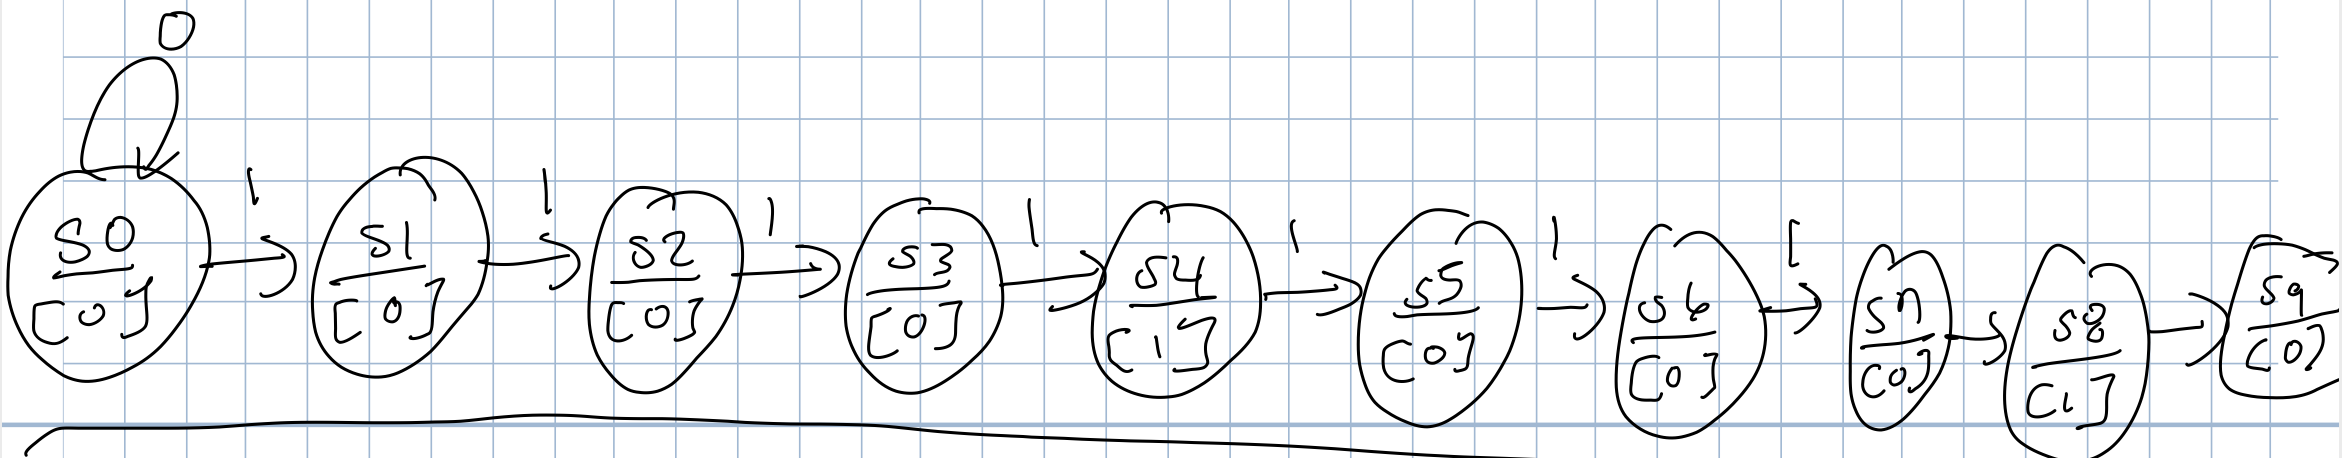
\includegraphics[width=\textwidth]{images/img1.png}
	\caption{\label{fig:moore_state_diagram}Moore State Diagram showing output at states 4 and 8.}
\end{figure}
\end{center}

\begin{table}[H]
\begin{center}
\begin{tabular}{| l | l | l |}
	\hline
	Bit & Label & Port \\ \hline
	clk & Clock & W5 \\ \hline
	enable & Switch 0 & V17 \\ \hline
	input & Switch 1 & U18 \\ \hline
	led0 & LED 15 & L1 \\ \hline
	state0 & LED 0 & U16 \\ \hline
	state1 & LED 1 & E19 \\ \hline
	state2 & LED 2 & U19 \\ \hline
	state3 & LED 3 & V19 \\ \hline
	state4 & LED 4 & W18 \\ \hline
	state5 & LED 5 & U15 \\ \hline
	state6 & LED 6 & U14 \\ \hline
	state7 & LED 7 & V14 \\ \hline
	state8 & LED 8 & V13 \\ \hline
	state9 & LED 9 & V3 \\ \hline
	output0 & Segment A & W7 \\ \hline
	output1 & Segment B & W6 \\ \hline
	output2 & Segment C & U8 \\ \hline
	output3 & Segment D & V8 \\ \hline
	output4 & Segment E & U5 \\ \hline
	output5 & Segment F & V5 \\ \hline
	output6 & Segment G & U7 \\ \hline
\end{tabular}
\caption{\label{tab:moore_state_ports}Port assignments for the Moore State Machine.}
\end{center}
\end{table}

\subsubsection{Results}
The state machine successfully progressed through the states and output '1' in states 4 and 8.

\subsection{Problem 3}

\subsubsection{Background}
Problem 3 will use the clock divider to test a Mealy State Machine acting as a sequence detector. A Mealy State Machine provides output depending on its current state and its input. This generally lowers the amount of states required to implement a state machine. This state machine should output '1' or HIGH when either "101" or "010" is detected by the input.

\subsubsection{Design Solution}


\subsubsection{Results}
The Mealy State Machine was able to successfully output '1' when "101" or "010" is detected.

\section{Conclusion}

\pagebreak

\textbf{Appendices}

\begin{appendices}

\section{Problem 1 VHDL Code}

\begin{lstlisting}[language=VHDL]
library IEEE;
use IEEE.STD_LOGIC_1164.ALL;
use IEEE.NUMERIC_STD.ALL;

entity Clockdivider is
     port(clk : in std_logic;
          start_timer : in std_logic;
	  FastClock,MediumClock,SlowClock, led0 : out std_logic);
end Clockdivider;

architecture clockdivider_arch of Clockdivider is

signal slowClock_sig : STD_LOGIC;

begin
    process  
    variable cnt :	std_logic_vector(26 downto 0):= 
    		"000000000000000000000000000";
    begin					 
        wait until ((clk'EVENT) AND (clk = '1'));
	       
		if (start_timer = '1') then
	       cnt := "000000000000000000000000000";
	    else  
           cnt := STD_LOGIC_VECTOR(unsigned(cnt) + 1);
	    end if;

   	    FastClock <= cnt(22);
   	    MediumClock <= cnt(24);	
   	    SlowClock <= cnt(26);
        slowClock_sig <= cnt(26);
	
        if (slowClock_sig = '1') then
		  led0 <= '1';
	    else
		  led0 <= '0';
	    end if;
	end process;
end clockdivider_arch;
\end{lstlisting}

\section{Problem 1 Constraints File}

\section{Problem 2 VHDL Code}
\begin{lstlisting}[language=VHDL]
library IEEE;
use IEEE.STD_LOGIC_1164.ALL;
use IEEE.NUMERIC_STD.ALL;

entity moore_machine is
    Port ( input : in STD_LOGIC;
           clk : in STD_LOGIC;
           enable : in STD_LOGIC;
           led0 : out STD_LOGIC;
           state : out STD_LOGIC_VECTOR(9 downto 0);
           output : out STD_LOGIC_VECTOR(6 downto 0));
end moore_machine;

architecture moore_arch of moore_machine is
component Clockdivider is
    Port ( clk : in STD_LOGIC;
           start_timer : in STD_LOGIC;
           FastClock,MediumClock,SlowClock,led0 : out STD_LOGIC);
end component Clockdivider;

signal slowClock : STD_LOGIC;
signal mediumClock : STD_LOGIC;
signal fastClock : STD_LOGIC;

begin
    clock : Clockdivider port map(clk, enable, slowClock, mediumClock,
    		fastClock, led0);
    

end moore_arch;
\end{lstlisting}

\section{Problem 2 Constraints File}

\section{Problem 3 VHDL Code}
\begin{lstlisting}[language=VHDL]

\end{lstlisting}

\section{Problem 3 Constraints File}

\end{appendices}
\end{document}
